Contextual language representations derived from Large Language Models (LLM) have led to impressive improvements in performance across many tasks in natural language processing, such as sentiment analysis, topic detection, and question answering. \\
In information retrieval, LLM based cross encoders and bi-encoder models have led to major improvements in relevance on benchmarking datasets like MSMARCO \cite{nguyen2016ms} and Natural Questions \cite{Kwiatkowski2019NaturalQA} and have been adopted as common backbones for many industrial deployments in search. Unlike traditional term-based search, contextual representations excel at semantic search, which can improve relevance as it matches intent instead of keywords. \\
\begin{figure}
    {\scalebox{0.45}{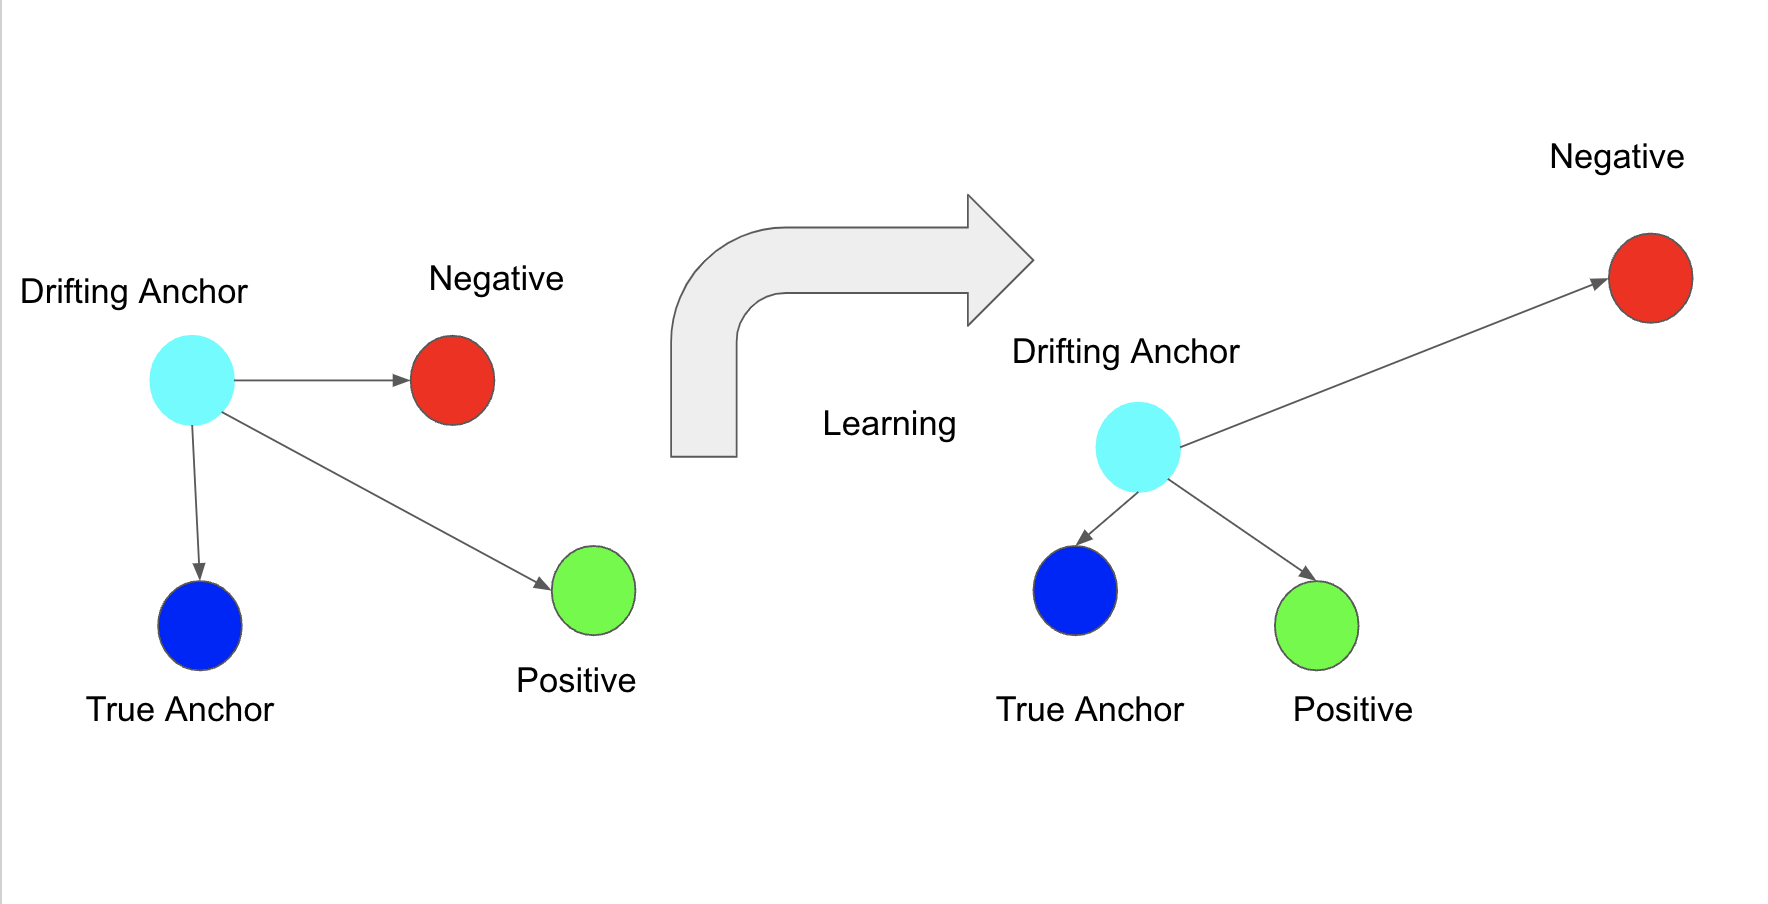
\includegraphics[width=\textwidth]{figure1.png}}}
  \caption{To learn a align the representation of queries and their counterparts with noise, a contrastive loss is used. Since the document encoder and its relative relation to the query encoder are frozen, an anchoring vector keeps the aligned encoder from drifting from its original learned representation.}
  \label{fig:fig1}
\end{figure}
While neural methods excel on well-formulated academic benchmarks, performance falters when faced with domain shifts or queries with misspellings or typos. On recent benchmarks like BEIR \cite{Thakur2021BEIRAH}, cross-encoders are more robust to shifts in domain than bi-encoders. \\
When looking at queries with some noise like typos and misspellings, the same holds \cite{zhuang-zuccon-2021-dealing}. Despite their superior performance on noisy queries and domain shifts, cross-encoder inference requirements make them too expensive to use at scale. \\
To avoid inference inefficiency of cross-encoder, bi-encoders have emerged as a popular method for retrieval, particularly for candidate generation in multi-stage ranking systems. Bi-encoders leverage query and document models trained to match their representations in a latent space. Since document representations are query independent, they only need to be generated once, and the inference load is limited to a single run of the query encoder. \\
Research on bi-encoder has been driven by the availability of large training datasets such as MSMARCO \cite{Campos2016MSMA}, Natural Questions (NQ)\cite{Kwiatkowski2019NaturalQA}, and Trivia QA (TQA) \cite{Joshi2017TriviaQAAL}. These datasets have allowed deep explorations on how to improve training procedure \cite{Qu2021RocketQAAO}, decrease index size \cite{Yamada2021EfficientPR}, and model efficiency \cite{Khattab2020ColBERTEA}.  Despite the tremendous success, these neural methods models are brittle to subtle search domain shifts and minor query formulation variations\cite{Wu2021AreNR}.  \\
While there has been plenty of work that has shown how neural methods are not robust to typos \cite{Wu2021AreNR} \cite{Penha2021EvaluatingTR} \cite{Sidiropoulos2022OnTI} \cite{Sidiropoulos2022AnalysingTR} \cite{zhuang-zuccon-2021-dealing}  all approaches which improve performance either require a new optimized general model such as CharBERT \cite{Zhuang2022CharacterBERTAS} or require retraining with data augmentation \cite{zhuang-zuccon-2021-dealing}. While effective, both approaches introduce a sizable overhead in dataset generation and augmentation or language model pre-training. Moreover, despite the effectiveness of these two techniques, further study is required to understand the interplay between data augmentation and  curriculum learning \cite{Mao2022CurriculumCC} and topic-aware sampling \cite{Hofsttter2021EfficientlyTA}. \\
\begin{table*}[htb!]
    \scalebox{0.60}{
    \begin{tabular}{|l|l|l|l|}
    \hline
        Noising Function & Alteration Type & Original & Alteration \\ \hline
        Determiner  & Syntactic & who sang waiting for a girl like you & who sang waiting a a girl like you \\ \hline
        Synonym & Semantic & \makecell{Which was the first European country to \\ abolish capital punishment?} & \makecell{Which was the first European country \\ to abolish majuscule punishment?}\\ \hline
        Lemmatize & Syntactic & who plays young dr mallard on ncis & who play young dr mallard on ncis \\ \hline
        Stemming & Syntactic & who recorded the song still the one? & who record the song still the one? \\ \hline
        Random Character Swap (RCS) & Surface & big little lies season 2 how many episodes & big litt e lies season 2 how many episodes \\ \hline
        Keyboard Character Swap (KCS) & Surface & when did veterans day start being called veterans day & when djid veterans day start being called veterans day \\ \hline
        Character Delete (CD) & Surface & when did big air snowboarding become an olympic sport & when did big air snowboarding become an olympic sort \\ \hline
        Reorder Word (RW) & Surface & who is the main character in green eggs and ham & who is the main character and green eggs in ham \\ \hline
        Back-Translation (BT) & Semantic & what is project charter in project management & What is a project charter in project management \\ \hline
        Paraphrasing & Semantic & turkey and china time difference & \makecell{Time difference between Turkey and China in the middle \\ of the night, depending on the time difference.} \\ \hline
    \end{tabular}}
    \caption{Example of the forms of query noise that we leverage to evaluate how robust bi-encoders are to noise.}
    \label{tab:query-noise}
\end{table*}
Seeking to improve the performance of the query encoder on noisy queries with high efficiency possible, we introduce \textbf{C}onstrastive \textbf{A}llignment \textbf{PO}st \textbf{T}raining (CAPOT). To avoid complicated dual encoder training regimes, CAPOT assumes that the document encoder and index are immutable and learn an improved query representation without altering existing relations to the index. As shown in figure \ref{fig:fig1}, CAPOT uses a traditional contrastive loss \cite{Schroff2015FaceNetAU} where queries with noise (positive samples) should be closer to the anchor (query without noise) than unrelated queries. Unlike a traditional contrastive loss, CAPOT introduces a notion of an anchoring loss between the unaltered model and the aligned model. As the model learns to group noisy queries with their unaltered roots, we also constrain its ability to alter the representation aligned with the unaltered document encoder.\\
The main contributions of our work are as follows:
\begin{itemize}
\item We introduce CAPOT, a highly efficient fine-tuning method for improving performance on noisy queries without retraining a model or index regeneration. 
\item We demonstrate that CAPOT is incredibly effective at making the encoder robust, particularly with typos. Using CAPOT approximates the impact of data augmentation without the associated computational overhead.
\item We demonstrate that CAPOT is robust enough to prove functional with completely unsupervised data. Using the ORCAS dataset, CAPOT can improve performance without access to the query training distribution.
\end{itemize}